% pour genree un pdf: faire
% pdflatex exemple.tex
\documentclass{article}

%% Paquets LateX utiles

\usepackage[utf8]{inputenc} 		% encodage des caracteres utilise (pour les caracteres accentues) -- non utilise ici.
%\usepackage[latin1]{inputenc} 		% autre encodage
\usepackage[french]{babel}		% pour une mise en forme "francaise"
\usepackage[T1]{fontenc} 
\usepackage{amsmath,amssymb,amsthm}	% pour les maths
\usepackage{graphicx}			% pour inclure des graphiques

\usepackage[hidelinks]{hyperref}
\usepackage{color}			% pour ajouter des couleurs dans vos textes
\usepackage{geometry}
\usepackage{tabularx}
\geometry{hmargin=2.5cm,vmargin=3cm}
\renewcommand{\contentsname}{\centering Contents}


\begin{document}
\begin{titlepage}
    \begin{flushleft}
    
\includegraphics[width=11em]{logo.png}\\[1.5cm]
    \end{flushleft}
    \begin{center}
        \textsc{{\LARGE \color{blue} Master Données, Apprentissage et Connaissances-DAC}}\\[5cm]
        \textsc{\Huge{RAPPORT PLDAC}}\\[1cm]
        \textbf{\Large{Sujet:}}
        \textsc{\large{Problème de clustering pour infrastructures sans fil.}}\\[6cm]
        \begin{minipage}{1\textwidth}
            \begin{flushleft} \large
            \textsc{\LARGE{Realisé par :}}\\[0.5cm]
            \textsc{Liticia TOUZARI}\\
            \textsc{Hanane DJEDDAL}\\[0.5cm]
            \textsc{Spécialité : DAC }\\ [1.5 cm]
            \end{flushleft}
        \end{minipage}
        \vfill
    \end{center}
  \end{titlepage}
  

\tableofcontents%  Table des matieres


\newpage

\vspace*{\stretch{0.5}}
  \begin{center}
\section*{\LARGE{Introduction}}
  \end{center}
\Large{\paragraph{}
        Aujourd'hui, le trafic de données sur les réseaux mobiles connaît une croissance explosive à mesure que les smartphones et tablettes compatibles avec Internet deviennent de plus en plus populaires.\\
Afin de répondre à la demande croissante de trafic de données, les opérateurs de réseaux mobiles doivent augmenter leur capacité de traitement de données, comme le déploiement de plus de stations de base et l'ajout d'unités de traitement de données supplémentaires aux stations de base. \\
Cependant, les dépenses en capital liées au déploiement de ces infrastructures de réseau deviennent de plus en plus élevées. Par conséquent, l'optimisation des dépenses d'investissement et des dépenses d'exploitation tout en maintenant une qualité de service est devenue une nécessité pour les opérateurs de réseaux mobiles.
\paragraph{}
Ce projet vise à mettre en œuvre des techniques de clustering afin de regrouper les ressources et infrastructures radio dans le but d'améliorer l'efficacité des services. 
Chaque ville est desservie par plusieurs nœuds sans fil qui sont géographiquement séparés; chacun d'eux est responsable d'une charge différente des appels vocaux, de la consommation multimédia et des messages provenant de différentes zones de la ville dans la journée. 
A ce jour, les différents nœuds d'accès  du réseau ne coopèrent pas, et chaque nœud est plutôt responsable de sa propre zone géographique. Les architectures futures des réseaux proposent de regrouper plusieurs stations sans fil et les traiter comme un ensemble avec un contrôleur commun, afin que les stations surchargées puissent être soutenues par des stations sous-chargées. 
\paragraph{}
Dans le cadre de ce projet, on proposera des méthodes de clustering efficaces, adaptées aux spécificités de l'environnement sans fil et des métriques des services de télécommunication. On utilisera des données fournies par l'opérateur Orange.
}
\vspace*{\stretch{1}}
\newpage

\section{Méthodes de Clustering}
\paragraph{}
Le clustering fait référence à un ensemble très large de techniques pour rechercher des sous-groupes, ou clusters, dans un ensemble de données. Lorsque nous regroupons les observations d'un ensemble de données, nous cherchons à les diviser en groupes distincts afin que les observations au sein de chaque groupe soient assez similaires les unes aux autres, tandis que les observations dans différents groupes sont assez différentes les unes des autres. Bien sûr, pour concrétiser cela, nous devons définir ce que signifie que deux ou plusieurs observations soient similaires ou différentes. En effet, il s'agit souvent d'une considération spécifique au domaine qui doit être faite sur la base de la connaissance des données étudiées.
Le clustering étant populaire dans de nombreux domaines, il existe un grand nombre de méthodes de clustering. Nous nous concentrons sur les deux approches de clustering les plus connues: le clustering K-means et le clustering hiérarchique. Dans le clustering K-means, nous cherchons à partitionner les observations en un nombre prédéfini de clusters. En revanche, dans le clustering hiérarchique, le nombre de clusters n'est pas prédéfini, nous nous retrouvons avec une représentation visuelle arborescente des observations, appelée dendrogramme, qui permet de visualiser immédiatement les regroupements obtenus pour chaque nombre possible de regroupements, de 1 à n. 
En général, nous pouvons regrouper des observations sur la base des caractéristiques afin d'identifier des sous-groupes parmi les observations, ou nous pouvons regrouper des caractéristiques sur la base des observations afin de découvrir des sous-groupes parmi les caractéristiques. [3]
\subsection{K-means Clustering} 
\paragraph{}
Le clustering K-means est une approche simple et élégante pour partitionner un ensemble de données en K clusters distincts qui ne se chevauchent pas. Pour effectuer le clustering K-means, nous devons d'abord spécifier le nombre souhaité de clusters K; alors l'algorithme K-means assignera chaque observation à exactement l'un des K clusters. 
La figure ci-dessous montre les résultats obtenus en déroulant l'algorithme sur l'ensemble des RRHs de Lille (ville Française) avec 88 emplacement différents.
\begin{flushleft}
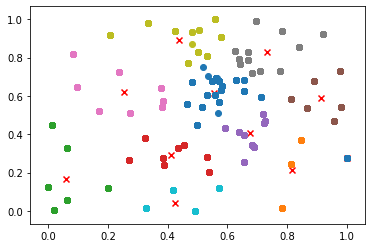
\includegraphics[width=20em]{images/k-means_lille.png}\\[1.5cm]
\end{flushleft}

La procédure de clustering K-means résulte d'un problème mathématique simple et intuitif. Nous commençons par définir une notation. Soit C1,. . . , CK désignent des ensembles contenant les indices des observations dans chaque cluster. Ces ensembles satisfont deux propriétés:
\begin{enumerate}
\item $C_{1} \cup C_{2} \cup ... \cup C_{k}=\lbrace1,...,n\rbrace$ chaque observation appartient à au moins l'un des K clusters.
\item $C_{k} \cap C_{k'}= \varnothing $ aucune observation n'appartient à plus d'un cluster.
\end{enumerate}
Par exemple, si la ième observation se trouve dans le kième groupe, alors $i \in C_{k}$. L'idée derrière le clustering K-means est qu'un bon clustering est celui pour lequel la variation intra-cluster est aussi petite que possible. La variation intra-cluster pour le cluster $C_{k}$ est une mesure $W(C_{k})$ de la différence entre les observations au sein d'un cluster. Par conséquent, nous voulons résoudre le problème :
$\min_{C_{1}, C_{2}, ... C_{K}}\sum^K_{k=1}C_{k}$. [3]

En termes, cette formule dit que nous voulons partitionner les observations en K clusters de telle sorte que la variation totale intra-cluster, additionnée sur tous les K clusters, soit aussi petite que possible.\\
Il s'agit en fait d'un problème très difficile à résoudre avec précision, car il existe presque $K^{n} $ façons de partitionner n observations en K clusters. Néanmoins, il existe un algorithme très simple pour fournir un optimum local - une assez bonne solution - au problème d'optimisation K-means. Cette approche est présentée dans le pseudo l'algorithme suivant :\\
\rule{\linewidth}{.1pt} 
\Large{Algorithme} K-means Clustering\\
\rule{\linewidth}{.1pt} 
\begin{enumerate}
\item Attribuez au hasard un numéro, de 1 à K, à chacune des observations.
Celles-ci servent d'initialisations.
\item Itérez jusqu'à ce que les affectations de cluster cessent de changer: 
\begin{enumerate}
\item Pour chacun des K clusters, calculer le centroïde du cluster.
\item Attribuez chaque observation au cluster dont le centroïde est le plus proche (où le plus proche est défini en utilisant la distance euclidienne par exemple).
\end{enumerate}
\end{enumerate}
\rule{\linewidth}{.1pt} 

Parce que l'algorithme K-means trouve une optimisation locale plutôt que globale, les résultats obtenus dépendront de l'affectation initiale (aléatoire) de chaque observation à l'étape 1 de l'algorithme. Pour cette raison, il est important d'exécuter l'algorithme plusieurs fois à partir de différentes configurations initiales aléatoires. Ensuite, en sélectionner la meilleure solution, c'est-à-dire celle pour laquelle l'objectif est le plus petit.\\
Comme vu précédemment, pour effectuer un clustering K-means, il faut définir le nombre de clusters K dés le départ. Le problème de la sélection de K est loin d'être simple. 

\vspace*{\stretch{0.5}}
\subsection{Clustering Hierarchique}
\paragraph{}
Un inconvénient potentiel de l'algorithme K-means est qu'il faut pré-spécifier le nombre de clusters K. Le clustering hiérarchique est une approche alternative qui ne nécessite pas un choix particulier de K. Le résultat du clustering est souvant traduit par une représentation arborescente attrayante des observations, appelée dendrogramme.\\

Le dendrogramme du clustering hiérarchique est obtenu via un algorithme extrêmement simple. Commençant par définir une sorte de mesure de dissimilarité entre chaque paire d'observations. Le plus souvent, la distance euclidienne est utilisée. L'algorithme se déroule de manière itérative. Partant du bas du dendrogramme, chacune des n observations est traitée comme son propre cluster. Les deux clusters qui se ressemblent le plus sont ensuite fusionnées pour qu'il y ait  n - 1 clusters. Ensuite, les deux clusters qui se ressemblent le plus sont fusionnés à nouveau, de sorte qu'il en reste  n - 2 clusters. L'algorithme procède de cette manière jusqu'à ce que toutes les observations appartiennent à un seul cluster et que le dendrogramme soit terminé.\\
L'algorithme de clustering hiérarchique est donné comme suit:\\
\rule{\linewidth}{.1pt} 
\Large{Algorithme} Clustering Hiérarchique\\
\rule{\linewidth}{.1pt} 
\begin{enumerate}
\item Commencez par n observations et une mesure (telle que la distance) et traitez chacun observation comme un cluster.
\item Pour i= n, n-1, ..., 2: 
\begin{enumerate}
\item Examinez toutes les dissemblances inter-cluster par paires parmi les i clusters et identifiez la paire de clusters qui sont les moins dissemblables (c'est-à-dire les plus similaires). Fusionnez ces deux clusters. La dissimilarité entre ces deux groupes indique la hauteur dans le dendrogramme à laquelle la fusion doit être placée.
\item Calculez les nouvelles dissemblances inter-cluster par paire parmi les i-1 clusters restants.
\end{enumerate}
\end{enumerate}
\rule{\linewidth}{.1pt}
\vspace*{\stretch{2}}
Le concept de dissimilarité entre une paire d'observations doit être étendu à une paire de groupes d'observations. Cette extension est obtenue en développant la notion de lien, qui définit la dissimilarité entre deux groupes d'observations. Les quatre types de liens les plus courants - complet, moyen, unique et centroïde - sont brièvement décrits dans le tableau ci-dessous:\\[0.5cm]
\begin{tabularx}{\linewidth}{|x|X|}
   \hline
  Linkage & Description  \\
  \hline
  Complet & Différenciation intercluster maximale. Calculez toutes les disparités par paires entre les observations du cluster A et les observations du cluster B, et retenir la plus grande de ces différences. \\
  \hline
  Unique & Dissimilarité intercluster minimale. Calculez toutes les disparités par paire entre les observations du cluster A et les observations du cluster B et noter la plus petite de ces différences. Un couplage unique peut entraîner des clusters étendues dans lesquelles des observations uniques sont fusionnées une par une. \\
  \hline
  Moyen & Dissimilarité intercluster moyenne. Calculez toutes les disparités par paires entre les observations du cluster A et les observations du cluster B et notez la moyenne de ces différences. \\
  \hline
  Centroïde & La dissimilarité entre le centroïde du cluster A et le centroïde du cluster B. La liaison centroïde peut entraîner des inversions indésirables. \\
  \hline
\end{tabularx}

\vspace*{\stretch{0.5}}
\begin{center}
\section*{\LARGE{Conclusion}}
   \end{center}
 \Large{\paragraph{}

 }
 \vspace*{\stretch{1}}
\end{document}